
This chapter is based on Refs. \cite{eli-daw-book}
and \cite{lich-book}.

\beq
\begin{array}{ll}
\text{root $\vec{\alp}$:}& [\vec{H},\;\cdot\;]E_{\vec{\alp}}
=
[\vec{H}, E_{\vec{\alp}}]= \vec{\alp} E_{\vec{\alp}}
\\
\text{weight $\vec{m}$:}&
\vec{H}\ket{j, \vec{m}}= \vec{m}\ket{j, \vec{m}}
\end{array}
\eeq

$\vec{\alp}, \vec{m}\in\RR^r$
where $r$ is the rank of the Lie algebra. $\RR^r$ is the root and weight space

$\ket{1}, \ket{2}, \ldots, \ket{n}\in \RR^n$ and
$H_i, E_\alp\in \RR^{n\times n}$  where s$n$ is
the dimension of the fundamental rep of the Lie algebra $\ger{su}(n)$

$\ket{j, \vec{m}}\in \CC^d$ where $d$ is the dimension of the irrep

\begin{figure}[h!]
\centering
\includegraphics[width=2.5in]
{weight-diagrams/weight-roots-relation.png}
\caption{Relationship between 2 weights $\vec{m}$ and $\vec{m}'$.}
\label{fig-weight-roots-relation}
\end{figure}

\begin{claim}
If 

\beq
\vec{H}\ket{\vec{m}}
=\vec{m}\ket{\vec{m}}
\eeq
then
\beq
\vec{H}E_{\vec{\alp}}\ket{\vec{m}}
=(\vec{m}+\vec{\alp})E_{\vec{\alp}}\ket{\vec{m}}
\eeq
\end{claim}
\proof
\beq
[\vec{H}, E_{\vec{\alp}}]=\vec{\alp}E_{\vec{\alp}}
\eeq
so
\beqa
\vec{H}E_{\vec{\alp}}\ket{\vec{m}}
&=&
E_{\vec{\alp}}\vec{H}\ket{\vec{m}} + \vec{\alp}E_{\vec{\alp}}\ket{\vec{m}}
\\&=&
(\vec{m}+\vec{\alp})E_{\vec{\alp}}\ket{\vec{m}}
\eeqa
\qed

\begin{claim}
For any weight $\vec{m}$ and
root $\vec{\alp}$,
if $k$ is an integer and

\beq k = -\;\frac{2\vec{m}\cdot \vec{\alp}}{\vec{\alp}\cdot\vec{\alp}}
\eeq
then

\beq
\vec{m}'=\vec{m} + k\vec{\alp}
\eeq
is a weight
with the same eigenvalue multiplicity as $\vec{m}$.
\end{claim}
\proof
\qed


\section{WD for $SU(2)$}


\beq
\ket{1}=\begin{pmatrix}
1
\\
0
\end{pmatrix}
,\quad
\ket{2}=\begin{pmatrix}
0
\\
1
\end{pmatrix}
\eeq

\beq
\sqrt{2}E_{12}=J_+=\ket{1}\bra{2},\quad
\sqrt{2}E_{-12}=E_{21}=J_- =\ket{2}\bra{1}
\eeq

\beq
J_z=\frac{1}{2}\left(
\ket{1}\bra{1}
-\ket{2}\bra{2}\right)
\eeq

\beq
\begin{array}{ll}
\bcen
\xymatrix{
&J_z\ar[dl]_{-J_-}
\ar[dr]^{J_+}
\\
J_-&&J_+\ar[ll]^{2J_z}
}
\ecen
&
\left\{
\begin{array}{l}
[J_+, J_-]=2J_z
\\
{[J_z, J_+]=J_+}
\\
{[J_z, J_-]=-J_-}
\end{array}\right.
\end{array}
\eeq



WD for irrep $j$, has weights $m$ where
\beq
J=j\in \left\{0, \frac{1}{2}, 1, \frac{3}{2}, \ldots\right\}
\eeq

\beq
J_z=j_z=m=\{-j, -j+1, \ldots, j-1, j\}
\eeq

$\ket{j,m}$ eigenvector of irrep $j$ with weight $m$

\section{WD for $SU(3)$}

\beq
\ket{1}=\begin{pmatrix}
1
\\
0
\\
0
\end{pmatrix}
,\quad
\ket{2}=\begin{pmatrix}
0
\\
1
\\
0
\end{pmatrix}
,\quad
\ket{3}=\begin{pmatrix}
0
\\
0
\\
1
\end{pmatrix}
\eeq

\beq
\sqrt{3}E_{12}=T_+=\ket{1}\bra{2},\quad
\sqrt{3}E_{-12}=E_{21}=T_- =\ket{2}\bra{1}
\eeq

\beq
\sqrt{3}E_{23}=U_+ = \ket{2}\bra{3},\quad
\sqrt{3}E_{-23}=E_{32} = U_- = \ket{3}\bra{2}
\eeq

\beq
\sqrt{3}E_{31}=V_+ = \ket{3}\bra{1},\quad
\sqrt{3}E_{-31}=E_{13}=V_- = \ket{1}\bra{3}
\eeq

\beq
T_z = \frac{1}{2}
\left(
\ket{1}\bra{1}
-\ket{2}\bra{2}\right),
\quad
U_z = \frac{1}{2}
\left(
\ket{2}\bra{2}
-\ket{3}\bra{3}\right)
,\quad
V_z = \frac{1}{2}
\left(
\ket{3}\bra{3}
-\ket{1}\bra{1}\right)
\eeq


\beq
\sqrt{\frac{3}{2}}H_1=T_z,
\quad
\sqrt{2}H_2=Y=
\frac{2}{3}
\left(
U_z-V_z
\right)
\eeq

{\bf isospin} $T_z\in \ZZ/2= 0, \pm\frac{1}{2}, \pm 1, \pm\frac{3}{2}, \pm 2, \ldots$

{\bf hypercharge} $Y\in \ZZ/3$


$H_1\in 
\frac{1}{\sqrt{6}}\ZZ$

$H_2\in \frac{1}{3\sqrt{2}}\ZZ$


\begin{figure}[h!]
\centering
\includegraphics[width=2.4in]
{weight-diagrams/123-vecs.png}
\caption{$\ket{1}, \ket{2}, \ket{3}$ 
vectors, and operators that act on them. $E_{-ij}=E_{ji}$ is in opposite direction 
as $E_{ij}$ for $i\ne j$ and $i,j=1,2,3$.}
\label{fig-123-vecs}
\end{figure}

\begin{figure}[h!]
\centering
\includegraphics[width=3.5in]
{weight-diagrams/tuv-plus.png}
\caption{Roots of $SU(3)$.}
\label{fig-tuv-plus}
\end{figure}



\renewcommand{\arraystretch}{1.5}
\beq
\begin{pmatrix}
\sqrt{\frac{3}{2}}H_1
\\
\sqrt{2}H_2
\end{pmatrix}
\ket{1}
=
\begin{pmatrix}
T_z
\\
Y
\end{pmatrix}
\ket{1}
=
\begin{pmatrix}
\frac{1}{2}
\\
\frac{1}{3}
\end{pmatrix}
\ket{1}
=
\vec{m}(1)\ket{1}
\eeq

\beq
\begin{pmatrix}
\sqrt{\frac{3}{2}}H_1
\\
\sqrt{2}H_2
\end{pmatrix}
\ket{2}
=
\begin{pmatrix}
T_z
\\
Y
\end{pmatrix}
\ket{2}
=
\begin{pmatrix}
-\frac{1}{2}
\\
\frac{1}{3}
\end{pmatrix}
\ket{2}
=
\vec{m}(2)\ket{2}
\eeq

\beq
\begin{pmatrix}
\sqrt{\frac{3}{2}}H_1
\\
\sqrt{2}H_2
\end{pmatrix}
\ket{3}
=
\begin{pmatrix}
T_z
\\
Y
\end{pmatrix}
\ket{3}
=
\begin{pmatrix}
0
\\
-\frac{2}{3}
\end{pmatrix}
\ket{3}
=
\vec{m}(3)\ket{3}
\eeq
\renewcommand{\arraystretch}{1}



\begin{figure}[h!]
\centering
\includegraphics[width=3.5in]
{weight-diagrams/weights-fundamental.png}
\caption{For $SU(3)$, roots in green and weights of fundamental rep in red.}
\label{fig-weights-fundamental}
\end{figure}






\section{$SU(3)$ examples}


one-to-one map of $SU(3)$ irreps and {\bf weight diagrams (WD)}

weights on the {\bf boundary of WD} are called {\bf dominant weights
}

nondegenerate weights are
represented by a single dot.
$k$-fold degenerate (i.e., eigenvalues with {\bf multiplicity} $k$) weights are represented by a dot with $k-1$ rings

WD are labelled by either by

\begin{itemize}
\item the dimension $d_{rep}$ of the irrep, with extra labels in case there are multiple irreps with the same dimension, 

\item the
$(\lam, \mu)$ WD-boundary dimensions. See Fig.\ref{fig-rep15}
\end{itemize}

One can show that


\beq
d_{rep}= \frac{1}{2}(\lam+1)(\mu+1)(\lam +\mu +2)
\label{eq-drep}
\eeq

For example, see Fig.\ref{fig-3-3star}. $SU(3)$ has 2 fundamental irreps, $\ul{3}$ and $\ul{3}^*$. Both are 3 dimensional. $(\lam,\mu)=(1,0)$ for $\ul{3}$, 
and $(\lam,\mu)=(0,1)$ for $\ul{3}^*$.
The formula Eq.(\ref{eq-drep}) for $d_{rep}$ gives 3 for both.




\begin{figure}[h!]
\centering
\includegraphics[width=2.9in]
{weight-diagrams/rep3.png}
\includegraphics[width=2.9in]
{weight-diagrams/rep3star.png}
\caption{WDs for the two fundamental irreps of $SU(3)$, $\ul{3}$ and $\ul{3}^*$. $(\lam,\mu)=(1,0)$ for $\ul{3}$, 
and $(\lam,\mu)=(0,1)$ for $\ul{3}^*$.}
\label{fig-3-3star}
\end{figure}


\begin{figure}[h!]
\centering
\includegraphics[width=3.5in]
{weight-diagrams/rep10.png}
\caption{WD for the $SU(3)$ irrep $\ul{10}$. $(\lam,\mu)=(3,0)$.}
\label{fig-rep10}
\end{figure}

\begin{figure}[h!]
\centering
\includegraphics[width=3.5in]
{weight-diagrams/rep8.png}
\caption{WD for the $SU(3)$ irrep $\ul{8}$. $(\lam,\mu)=(1,1)$.}
\label{fig-rep8}
\end{figure}

\begin{figure}[h!]
\centering
\includegraphics[width=3.5in]
{weight-diagrams/rep15.png}
\caption{WD for the $SU(3)$ irrep $\ul{15}$. $(\lam,\mu)=(2,1)$.}
\label{fig-rep15}
\end{figure}

\hrule
{\bf An aside about hypercharge}

Several different quantum numbers are called hypercharge in particle physics. For example, in the
Gell-mann-Nishijima relation
\beq Q= T_z + \frac{1}{2}Y'\eeq
hyperchage= $Y'\in \ZZ$, isospin= $T_z\in \ZZ/2$, so charge= $Q\in\ZZ/2$. For example,
for nucleons, 
\beq \text{proton (p)}: \quad T_z=\frac{1}{2},\quad Y'=1\implies Q=1\eeq
\beq\text{neutron (n)}: \quad T_z=-\;\frac{1}{2},\quad Y'=1\implies Q=0\eeq
As a mnemonic, remember that a nucleon has 3 quarks with $Y=1/3$,
and $Y'$ for the nucleon is the sum of $Y$ for each quark. $Y=1/3$ for up or down quarks, and $Y=-2/3$ for the strange quark. $u,d$ constitute an $SU(2)$ doublet and $s$ an $SU(2)$ singlet.

\section{Relation of weights of WD to Semi-Standard Young Tableau}



Given a young diagram YD, a SYT/SSYT (Standard or Semi-Standard Young Tableau) 
for the YD satisfies


\begin{itemize}
\item Rows strictly/weakly increasing
\item Columns strictly increasing
\item Entries in $\{1,2,\dots, n\}$.
$n=3$ for $SU(3)$
\end{itemize}
Thus, SYT/SSYT disallow/allow repetitions along a row.

SYT are used, for example, to label the irreps of $S_n$.
Hence, there is a 1-1 relation between Young Symmetrizer operators
and STY. 


SSYT are used below to label the basis vectors of an irrep of $SU(n)$.

SYT \xymatrix{\ar[r]_{\text{1 to 1}}&} Young operators, SSYT \xymatrix{\ar[r]_{\text{1 to 1}}&} weights of WD



There is a 1-1 relationship between YD and WD,
and a 1-1 relationship between the SSYT of a YD and the 
weights of the corresponding WD.
Degenerate weights have different SSYT.


\beq
(t_z,y)=
\sum_{\text{boxes}}
\left\{
\begin{array}{ll}
(\frac{1}{2},\frac{1}{3}), & \text{for each 1 box}\\
(-\frac{1}{2},\frac{1}{3}), & \text{for each 2 box}\\
(0,-\frac{2}{3}), & \text{for each 3 box}
\end{array}
\right.
\eeq

\beq
t_z=
\frac{1}{2}(n_1-n_2)
\eeq

\beq 
y=\frac{1}{3}(n_1 + n_2 - 2 n_3)
\eeq
\hrule
SU(3) octet example. 


Young diagram for the octet ($\ul{8}$, (1,1), Fig.\ref{fig-rep8})

$$
\ydiagram{2,1}
$$

\beq
\caly = S_{12}A_{13}= [1+(12)][1-(13)]
\eeq

\beqa\ket{\psi}=
\caly\ket{a}\ket{b}\ket{c}
&=&
S_{12}\left(
\ket{a}\ket{b}\ket{c}-\ket{c}\ket{b}\ket{a}
\right)
\\&=&
[\ket{a}\ket{b}\ket{c} + \ket{b}\ket{a}\ket{c}]
-[\ket{c}\ket{b}\ket{a}+\ket{c}\ket{a}\ket{b}]
\eeqa

\begin{enumerate}

\item
\beq 
\begin{array}{l|l|l}
\begin{ytableau}
1 & 1\\
2
\end{ytableau}
&
(t_z,y)=\left(+\tfrac12,1\right)
&\ket{\psi} \text{ with } abc\rarrow u_1
u_1 u_2
\end{array}
\eeq 

\item

\beq 
\begin{array}{l|l|l}
\begin{ytableau}
1 & 2\\
2
\end{ytableau}
&
(t_z,y)=\left(-\tfrac12,1\right)
& \ket{\psi} \text{ with } abc\rarrow u_1 u_2 u_2
\end{array}
\eeq 


\item
\beq
\begin{array}{l|l|l}
\begin{ytableau}
1 & 1\\
3
\end{ytableau}
&
(t_z,y)=(+1,0)
&
\ket{\psi} \text{ with } abc\rarrow u_1 u_1 u_3
\end{array}
\eeq 

\item
\beq
\begin{array}{l|l|l}
\begin{ytableau}
1 & 2\\
3
\end{ytableau}
&
(t_z,y)=(0,0)
&
\ket{\psi} \text{ with } abc\rarrow u_1 u_2 u_3
\end{array}
\eeq 

\item

\beq 
\begin{array}{l|l|l}
\begin{ytableau}
2 & 2\\
3
\end{ytableau}
&
(t_z,y)=(-1,0)
&
\ket{\psi} \text{ with } abc\rarrow u_2 u_2 u_3
\end{array}
\eeq 


\item 

\beq 
\begin{array}{l|l|l}
\begin{ytableau}
1 & 3\\
2
\end{ytableau}
&
(t_z,y)=(0,0)
&\ket{\psi} \text{ with } abc\rarrow u_1 u_3 u_2
\end{array}
\eeq 


\item

\beq 
\begin{array}{l|l|l}
\begin{ytableau}
1 & 3\\
3
\end{ytableau}
&
(t_z,y)=\left(+\tfrac12,-1\right)
&
\ket{\psi} \text{ with } abc\rarrow u_1 u_3 u_3
\end{array}
\eeq 

\item

\beq 
\begin{array}{l|l|l}
\begin{ytableau}
2 & 3\\
3
\end{ytableau}
&
(t_z,y)=\left(-\tfrac12,-1\right)
& \ket{\psi} \text{ with } abc\rarrow u_2 u_3 u_3
\end{array}
\eeq 

\end{enumerate}

\begin{figure}[h!]
\centering
\includegraphics[width=3.5in]
{weight-diagrams/rep8-with-yt.png}
\caption{WD for the $SU(3)$ octet with YT
for each weight.}
\label{fig-rep8-with-yt}
\end{figure}